\documentclass[a4paper, czech]{article}

\usepackage[czech]{babel}
\usepackage{indentfirst}
\usepackage{graphicx}
\usepackage{float}
\usepackage[margin=1.5cm]{geometry}
\usepackage{booktabs}
\usepackage{amsmath}
\usepackage{caption}
\usepackage{subcaption}
\usepackage{siunitx}
\usepackage{accents}


\title{Úloha č.2: Dioda jako usměrňovač a řízený odpor}
\author{Karolína Andrea Šebestová}
\date{Datum měření: 29.2.2024}

\begin{document}

\maketitle

\section{Teoretický úvod}
\subsection{Dioda jako usměrňovač}

Schopnost diody vést proud pouze jedním směrem se využívá
v diodových usměrňovačích. Jednocestný usměrňovač na Obr. 1
propouští pouze kladnou polaritu napětí z generátoru G.

Závěrná zotavovací doba diody $trr$
(Reverse Recovery, viz Obr. 2)
je dynamickým parametrem, který udává, za jak dlouho dioda dokáže přejít z
propustného do závěrného režimu. Při změně polarity napětí na diodě pokles
proudu pokračuje i do záporných hodnot, protože dochází k postupnému
odčerpávání injektovaných minoritních nosičů náboje, které se v diodě
nahromadily při propustné polarizaci. Dioda se tedy stává nevodivou až po
uplynutí doby závěrného zotavení $trr$.

\begin{figure}[H]
    \centering
    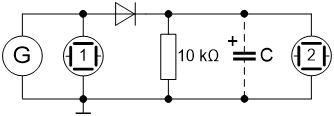
\includegraphics{obr1.png}
    \caption{Zapojení sériového usměrňovače}
\end{figure}
\begin{figure}[H]
    \centering
    \begin{subfigure}[b]{0.49\textwidth}
        \centering
        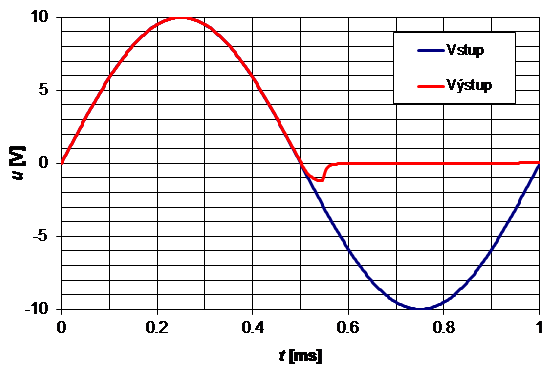
\includegraphics[width=\textwidth]{obr2-1.png}
    \end{subfigure}
    \begin{subfigure}[b]{0.49\textwidth}
        \centering
        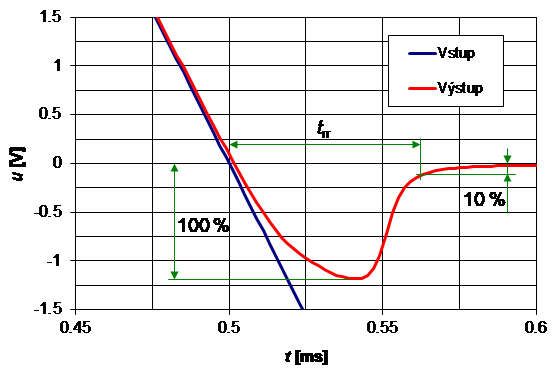
\includegraphics[width=\textwidth]{obr2-2.png}
    \end{subfigure}
    \caption{Ilustrační průběhy pro určení závěrné zotavovací doby diody}
\end{figure}

\subsection{Dioda jako řízený odpor}

Statický odpor diody v propustném směru je dán podílem
napětí a proudu na diodě $R_S = U_F\ /\ I_F$.
Dynamický odpor je dán strmostí V-A charakteristiky (např. Obr. 2),
tedy derivací proudu podle napětí $R_D
= du_F\ /\ di_F$. Změnu odporu diody lze realizovat
přivedením stejnosměrného řídicího napětí $U_R$,
viz Obr. 3.
Tím se pro střídavé napětí z generátoru mění dělicí poměr odporového
děliče tvořeného diodou a rezistorem $10 k\Omega$. Napětím $U_R$ lze takto elektronicky řídit přenos
obvodu, tedy poměr amplitud $U_2\ /\ U_1$.

\begin{figure}[H]
    \centering
    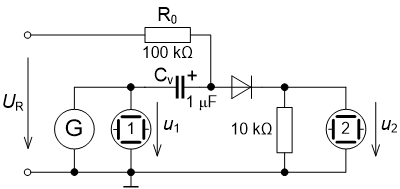
\includegraphics{obr3.png}
    \caption{Zapojení s diodou jako řízeným odporem}
\end{figure}

\section{Seznam přístrojů}

\begin{enumerate}
    \item Generátor Agilent 33521A
    \item Zdroj Agilent E3620A
    \item Osciloskop Agilent DSO-X 2002A
    \item Osciloskopická sonda HP 10074B
\end{enumerate}

\section{Úkoly měření}

\begin{enumerate}
    \item Ve všech
úkolech této laboratorní úlohy použijte diody 1N4148. Sestavte obvod podle Obr. 3. Na generátoru nastavte sinusový průběh o kmitočtu
1 kHz s mezivrcholovou hodnotou napětí 20 Vpp (pp značí peak-peak,
tedy špička-špička). Ve skutečnosti však na generátoru nastavte 10 Vpp,
čímž vlivem vysoké vstupní impedance obvodu na Obr. 3 získáte na výstupu generátoru požadovaných cca 20 Vpp.
U generátoru je nutné pro aktivaci výstupu stisknout tlačítko Channel a poté
tlačítkem pod displejem nastavit Output on. Tlačítko Channel musí být
prosvětleno. Do kanálu 2 osciloskopu přivádějte výstupní napětí obvodu pomocí
osciloskopické sondy s dělicím poměrem napětí 10:1. To platí pro všechny
úkoly měření v této úloze. Ve všech úkolech je také třeba připojovat černé
krokodýlky koaxiálních kabelů a sondy k zemnímu, tedy ve schématu
spodnímu, vodiči. Aby osciloskop se sondou ukazoval správné napěťové hodnoty, zmáčkněte
na osciloskopu tlačítko čísla kanálu 2, poté pod displejem Probe a
v položce Probe nastavte pomocí kolečka s prosvětlenu šipkou 10.0:1.
Zobrazte na osciloskopu průběhy vstupního a výstupního napětí obvodu tak, aby
byly vidět zhruba dvě periody signálu. Tyto průběhy vložte (jako čitelnou fotku
obrazovky nebo uložením na USB) či obkreslete do protokolu.
    \item Nastavení
generátoru ponechte z předchozího bodu a osciloskop nastavte tak, aby
zobrazoval cca 5 period signálu. Na výstup usměrňovače připojte dle Obr. 3
filtrační kondenzátor o kapacitě C = 100 nF a
poté $1\ \mu F$ a vložte do protokolu průběhy z osciloskopu, které vzájemně porovnejte.
    \item Sestavte
zapojení s diodou jako řízeným odporem podle Obr. 3.3.
Výstupní napětí z generátoru $U_1$
volte 100 mVpp (na generátoru tedy nastavujte 50 mVpp), jeho
frekvenci 1 kHz, průběh sinus. Změřte a v protokolu vyneste do grafu přenos
napětí $A_{dB} = 20log(U_2/U_1)$
obvodu jako funkci řídicího napětí $U_R$.
Veličiny $U_1$ a $U_2$ jsou mezivrcholové hodnoty vstupního a
výstupního napětí $u_1$, $u_2$, které měřte osciloskopem pomocí funkce
tlačítka Meas. Tlačítkem Type pod displejem zvolte Peak-Peak a tlačítkem Source
vyberte měřený kanál, volbu potvrďte pomocí Add Measurement. Vstup 2 osciloskopu
je přepnut na střídavou vazbu AC, což provedete stiskem tlačítka čísla kanálu
2, poté tlačítkem pod displejem Coupling vyberete AC. Napětí $U_R$ nastavujte na zdroji E3620A od 0 do 4 V minimálně
v 16 hodnotách, přičemž pro malá $U_R$
volte jemnější krok.
\end{enumerate}

\newpage

\section{Naměřené a vypočtené hodnoty}

\subsection{Sériový usměrňovač bez kondenzátoru}

Sériový usměrňovač byl zapojen bez kondenzátoru a jeho vstupní a výstupní průběhy byly zobrazeny na osciloskopu. Vstupní signál je zobrazen \underline{žlutou} barvou a výstupní signál je zobrazen barvou \underline{zelenou}. Na zobrazeném průběhu je dobře vidět, že vstupní signál má tvar sinusoidy, zatímco výstupní signál vypadá podobně, avšak záporná půlperioda průběhu je vynulována a signál je tak usměrněný.

\begin{figure}[H]
    \centering
    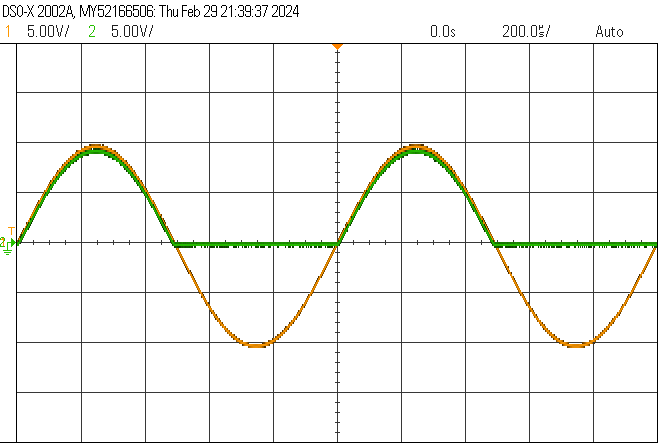
\includegraphics[width=0.7\textwidth]{scope_1.png}
    \caption{Naměŕené průběhy sériového usměrňovače \underline{bez kondenzátoru}}
\end{figure}

\subsection{Sériový usměrňovač s kondenzátorem}

Do stejného zapojení jsme připojili kondenzátor s kapacitou $100\ nF$. Ten se v první kladné půlperiodě nabije a poté se postupně vybíjí, dokud nedojde k jeho opětovnému nabití následující kladnou půlperiodou. Dochází tedy k částečnému vyhlazení výstupního průběhu.

\begin{figure}[H]
    \centering
    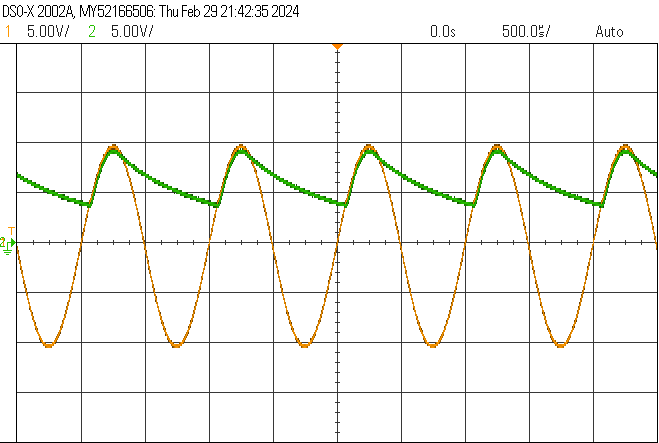
\includegraphics[width=0.7\textwidth]{scope_2.png}
    \caption{Naměřené průběhy sériového usměrňovače s kondenzátorem \textbf{100 nF}}
\end{figure}

\newpage

V tom samém zapojení jsme kondenzátor nahradili jiným s kapacitou $1\ \mu F$. Pozorujeme, že došlo ke stejnému jevu jako v předcházejícím případě, ale výstupní průběh je ještě více vyhlazen.

\begin{figure}[H]
    \centering
    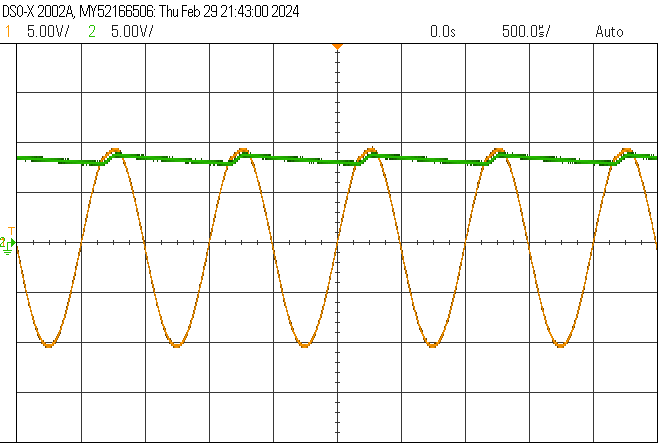
\includegraphics[width=0.7\textwidth]{scope_3.png}
    \caption{Naměřené průběhy sériového usměrňovače s kondenzátorem \textbf{1 uF}}
\end{figure}

\subsection{Dioda jako řízený odpor}

Naměřené i vypočtené hodnoty jsme vynesli do jedné společné tabulky.

Slovní popis symbolů veličin: $n$ - pořadí měření; $U_R$ - stejnosměrné řídící napětí; $U_1$ - mezivrcholová hodnota vstupního napětí; $U_2$ mezivrcholová hodnota výstupního napětí; $A_{dB}$ - napěťový přenos obvodu

\begin{table}[H]
\centering
\begin{tabular}{lS[table-format=1.2, locale = DE]ccS[table-format=3.3, round-mode = places, round-precision = 3, locale = DE]}
\toprule
$n$ & {$U_R\ (V)$} & $U_1\ (mVpp)$ & $U_2\ (mVpp)$ & {$A_{dB}\ (dB)$}      \\
\midrule
1                     & 0      & 105     & 11      & -19,59593228  \\
2                     & 0,1    & 105     & 12      & -18,84016106  \\
3                     & 0,2    & 105     & 14      & -17,50122527  \\
4                     & 0,25   & 105     & 16      & -16,34138633  \\
5                     & 0,3    & 105     & 19      & -14,84871396  \\
6                     & 0,4    & 105     & 27      & -11,7965107   \\
7                     & 0,5    & 105     & 35      & -9,542425094  \\
8                     & 0,6    & 105     & 42      & -7,958800173  \\
9                     & 0,75   & 105     & 51      & -6,272382459  \\
10                    & 1      & 105     & 61      & -4,717189281  \\
11                    & 1,25   & 105     & 71      & -3,398619007  \\
12                    & 1,5    & 105     & 76      & -2,807514136  \\
13                    & 1,75   & 105     & 80      & -2,361986242  \\
14                    & 2      & 105     & 84      & -1,93820026   \\
15                    & 2,25   & 105     & 87      & -1,633400929  \\
16                    & 2,5    & 105     & 88      & -1,534132538  \\
17                    & 2,75   & 105     & 90      & -1,338935793  \\
18                    & 3      & 105     & 92      & -1,148029434  \\
19                    & 3,25   & 105     & 93      & -1,05412701   \\
20                    & 3,5    & 105     & 95      & -0,869313876  \\
21                    & 3,75   & 105     & 95      & -0,869313876  \\
22                    & 4      & 105     & 96      & -0,778361321  \\
\bottomrule
\end{tabular}
\caption{Naměřené a vypočtené hodnoty přenosové charakteristiky diody 1N4148}
\end{table}

\newpage

\section{Příklady výpočtu}
Přenos napětí obvodu $A_{dB}$ byl vypočten podle následujícího vztahu:
$$A_{dB}=20 \cdot \log\left(\frac{U_2}{U_1}\right)$$

Uvedeme si konkrétní příklad výpočtu pro první řádek tabulky naměřených hodnot:
$${A_{dB}}_1 = 20 \cdot \log\left(\frac{U_2}{U_1}\right) = 20 \cdot \log\left(\frac{11 \cdot 10^{-3}V}{105 \cdot 10^{-3}V}\right) \approx \underline{\underline{-19,596}}$$

\section{Grafy}

Naměřené hodnoty napěťového přenosu $A_{dB}$ byly vyneseny do grafu jako funkce stejnosměřného řídícího napětí $U_R$. Výsledný graf tedy tvoří přenosovou charakteristiku.

\begin{figure}[H]
    \centering
    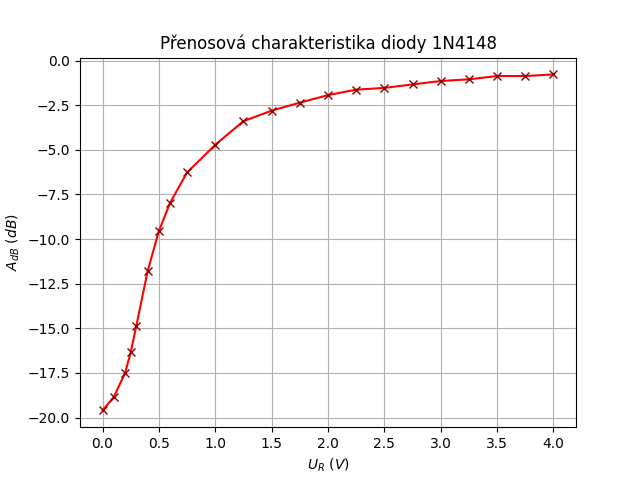
\includegraphics[width=0.8\textwidth]{graf.png}
    \caption{Grafické znázornění přenosové charakteristiky diody 1N4148}
\end{figure}

\section{Závěr}

V prvním zapojení jsme pozorovali schopnost diody vést proud pouze jedním směrem. Naše zapojení propouštělo pouze kladnou půlperiodu vstupního signálu z generátoru. To proto, že v kladné půlperiodě je dioda zapojena v prospustném směru, ale v záporné půlperiodě je zapojena v závěrném směru.

Čas, za který dioda přejde z propustného do závěrného režimu nazýváme \textit{závěrná zotavovací doba diody} $t_{rr}$. Pokles proudu při změně polarity pokračuje i do záporných hodnot, tento jev je však zanedbatelný. Tento jev trvá tak krátko, že se nám ho v našich podmínkách pro měření nepodařilo pozorovat a proto jsme se ním nezabývali.

Při připojení filtračního kondenzátoru do obvodu sériového usměrňovače jsme pozorovali částečné vyhlazení výstupního napěťového průběhu. Tento jev je způsoben tím, že kondenzátor se v první kladné půlperiodě nabije na maximální hodnotu kladného napětí a poté se postupně vybíjí dokud nedojde k jeho opětovnému nabití následující kladnou půlperiodou. Pozorovali jsme také, že připojením filtračního kondenzátoru s větší kapacitou jsme dosáhli mnohem lepšího vyhlazovacího jevu. To je způsobeno menším poklesem napětí na kondenzátoru s větší kapacitou při jeho vybíjení.

Na druhém zapojení jsme pozorovali možnost elektronicky řídit přenos (neboli poměr napětí $U_2/U_1$) diody pomocí řídícího napětí $U_R$. V tomto zapojení se dioda chová jako řízený odpor. Celé zapojení je tedy v podstatě odporový dělič napětí tvořen samotnou diodou a rezistorem. Změnou řídícího napětí $U_R$ jsme schopni měnit poměr odporového děliče. Závislost přenosu obvodu $A_{dB}$ na řídícím napětí $U_R$ je možné vidět v grafu přenosové charakteristiky.

\end{document}
